\documentclass[11pt]{article}
\usepackage{color}
\usepackage[usenames,dvipsnames,svgnames,table]{xcolor}
\definecolor{dark-red}{rgb}{0.7,0.1,0.1} 
\definecolor{dark-blue}{rgb}{0,0,0.7} 
\usepackage[linkcolor=dark-red,
            colorlinks=true,
            urlcolor=dark-blue,
            pdfstartview={XYZ null null 1.00},
            pdfauthor={Gaurav Sood, gsood07@gmail.com},
            citecolor=dark-red,
            bookmarks=false,
            pdfborder={0 0 0},
            pdftitle={The Review}]{hyperref}
            
\usepackage{amsfonts,amssymb,amsbsy,amsmath,amsxtra}

\usepackage{indentfirst}
\usepackage{setspace} % To set line spacing
\usepackage{multirow}

\usepackage{verbatim}

\usepackage[multiple]{footmisc}
\usepackage{fancyvrb}

\usepackage{longtable}

\usepackage[margin=1in]{geometry}
\usepackage{graphicx}

\raggedright
\parindent=1.5em % <- or whatever indent you want

\usepackage{natbib}
\usepackage{url}
\begin{comment}

setwd(paste0(githubdir, "/meta_apsr/ms/"))	
tools::texi2dvi("the_review.tex", pdf=TRUE, clean=TRUE)	
setwd(paste0(githubdir, "/meta_apsr/"))

\end{comment}

\begin{document}
\title{\vspace{-1cm}\normalsize{\textbf{The Review: Production and Consumption of APSR Articles}}}
\author{Gaurav Sood\\\small{\href{mailto:gsood07@gmail.com}{\tt{gsood07@gmail.com}}}}
\maketitle
\begin{center}
\vspace{-.5cm}\textbf{NB:} Preliminary draft. Please do not cite without permission.
\end{center}
\vspace{.2cm}
\doublespacing

Scientific production is affected by a variety of variables that have little to do with the science. Availability of funding, fads, various parts of the scientific paper production pipeline: (artificial) limits on journal space, the number of articles editors must review, the incentives to be nice to the author, etc., among other things, affects what topic is researched, the quality of research, and who produces and reads it, among other things. Using data on all articles published in the The American Political Science Review, the preeminent journal in political science since its inception nearly a hundred years ago, I shed light on some of those issues in political science.\footnote{The data and scripts to acquire, process and analyze the data can be downloaded from \href{https://github.com/soodoku/meta_apsr}{https://github.com/soodoku/meta\_apsr}.} 

Over the past 100 or so years, article length has shown marked variability (see Figure~\ref{fig:pages}). There is a marked see-saw pattern in the average length of the article, but unlike top economics journals we don't see a marked trend towards longer articles \citep{card2013nine, card2014page}. (It is very likely, however, that the length of online appendices has grown substantially.)

Over time, the number of articles per issue has shown a sharp increase --- over 100 years, the number of articles has more than doubled (see Figure~\ref{fig:narticles}). (Though, over the past thirty or so years, the number of articles per issue has remained steady.) 

Given the two things we find above, it is obvious that pages per issue would have increased. And so we find (see Figure~\ref{fig:issue}). 

Looking at production, I tallied two features: number of authors per article over time, and proportion of female authors per article over time. Like with other sciences, co-authorship is on the rise. Though, solo authored papers still make a sizable proportion of publications in the APSR, the modal publication today has two authors (see Figure~\ref{fig:nauthors}).

The data on proportion of women authors per article is distressing. While again the proportion of women on each article published in the APSR has been rising, the average article still has just 20\% female authors (see Figure~\ref{fig:women}).  

Flipping the lens and looking at two consumption metrics: number of abstract views and number of full-text views, provides a familiar power-law distribution. Most of the articles (abstracts) aren't viewed at all. And a small set of articles gets a lot of views (see Figures~\ref{fig:abstracts} and ~\ref{fig:fulltext}). .

Lastly, for some fun. Some previous analysis suggests that paper titles have gotten longer over time.\footnote{See \href{http://datacolada.org/2013/12/04/titleogy/}{http://datacolada.org/2013/12/04/titleogy/}} Here I plot the length of title of APSR articles over time. It appears the average title length has increased by 50\% --- from an average of 50 to about 75 characters today.

\clearpage
\begin{center}
\large{Figures}
\end{center}

\begin{figure}[htbp]
\centering
\caption{Number of Pages per Article Over Time}
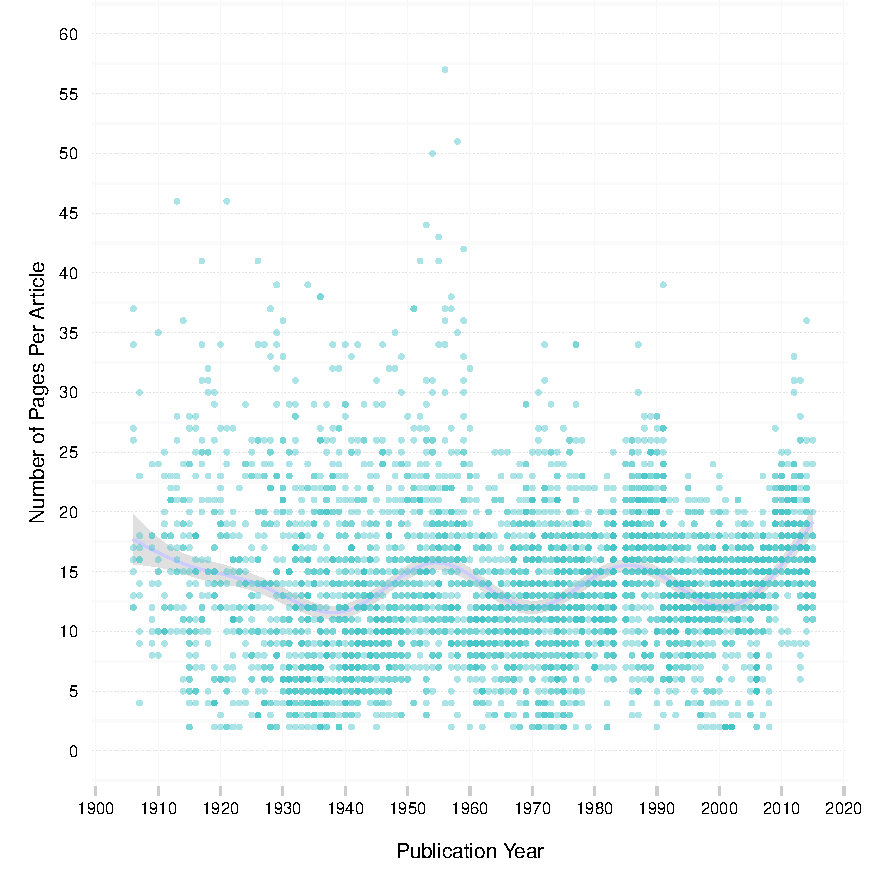
\includegraphics[scale=.85]{../figs/n_pages_per_article_over_time.pdf}
\label{fig:pages}
\end{figure}

\begin{figure}[htbp]
\centering
\caption{Number of Articles per Issue Over Time}
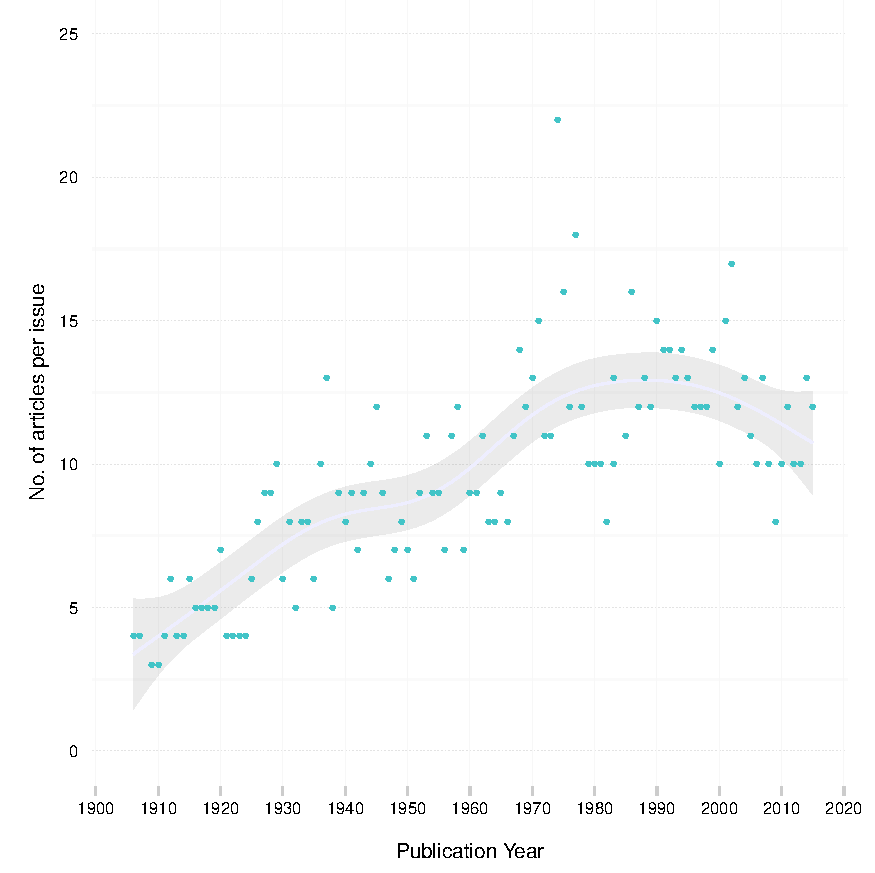
\includegraphics[scale=.85]{../figs/articles_per_issue_over_time.pdf}
\label{fig:narticles}
\end{figure}

\begin{figure}[htbp]
\centering
\caption{Pages per Issue Over time}
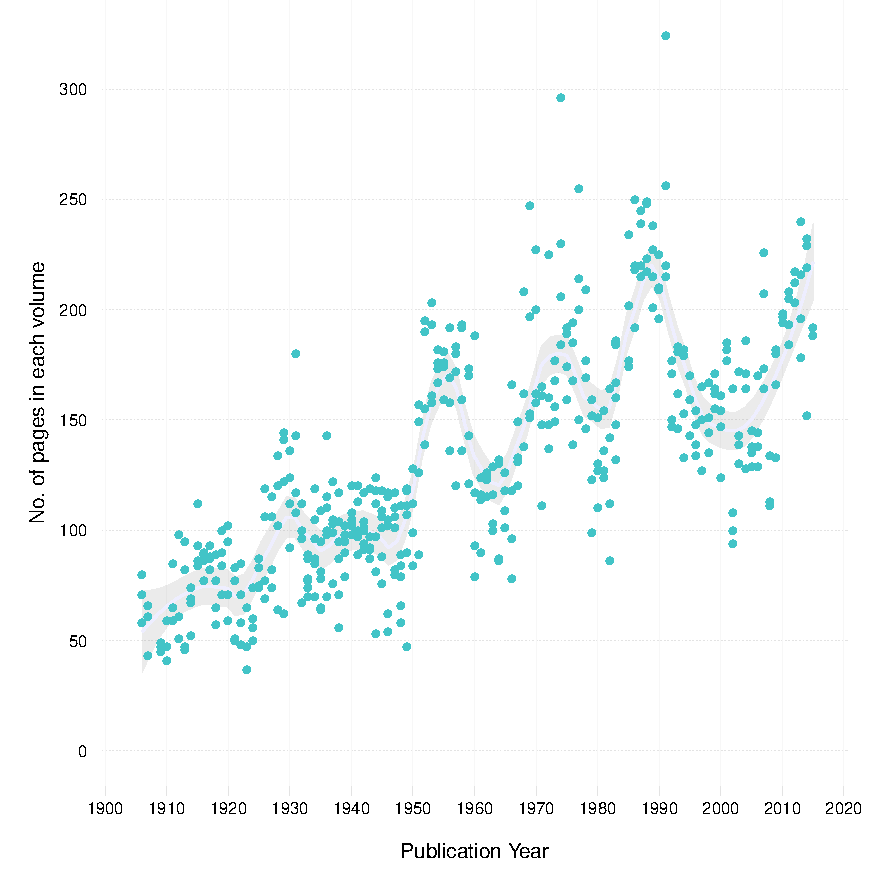
\includegraphics[scale=.85]{../figs/pages_per_issue_over_time.pdf}
\label{fig:issue}
\end{figure}

\begin{figure}[htbp]
\centering
\caption{Number of Authors per Article Over Time}
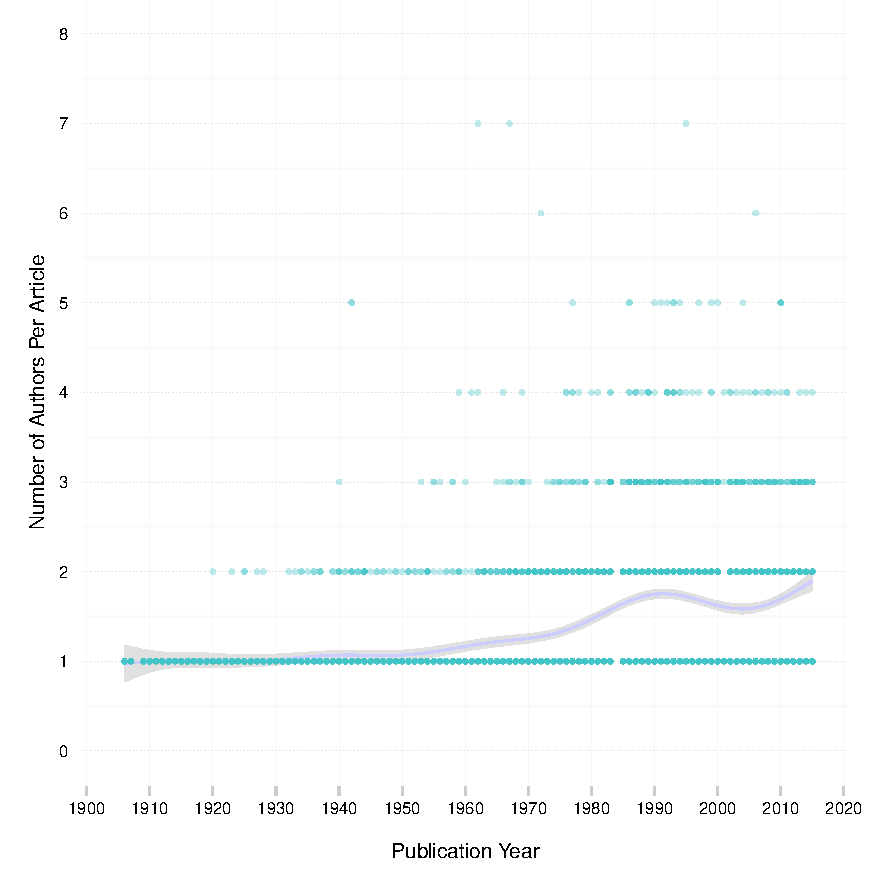
\includegraphics[scale=.85]{../figs/n_authors_per_article_over_time.pdf}
\label{fig:nauthors}
\end{figure}

\begin{figure}[htbp]
\centering
\caption{Proportion of Women Per Article Over Time}
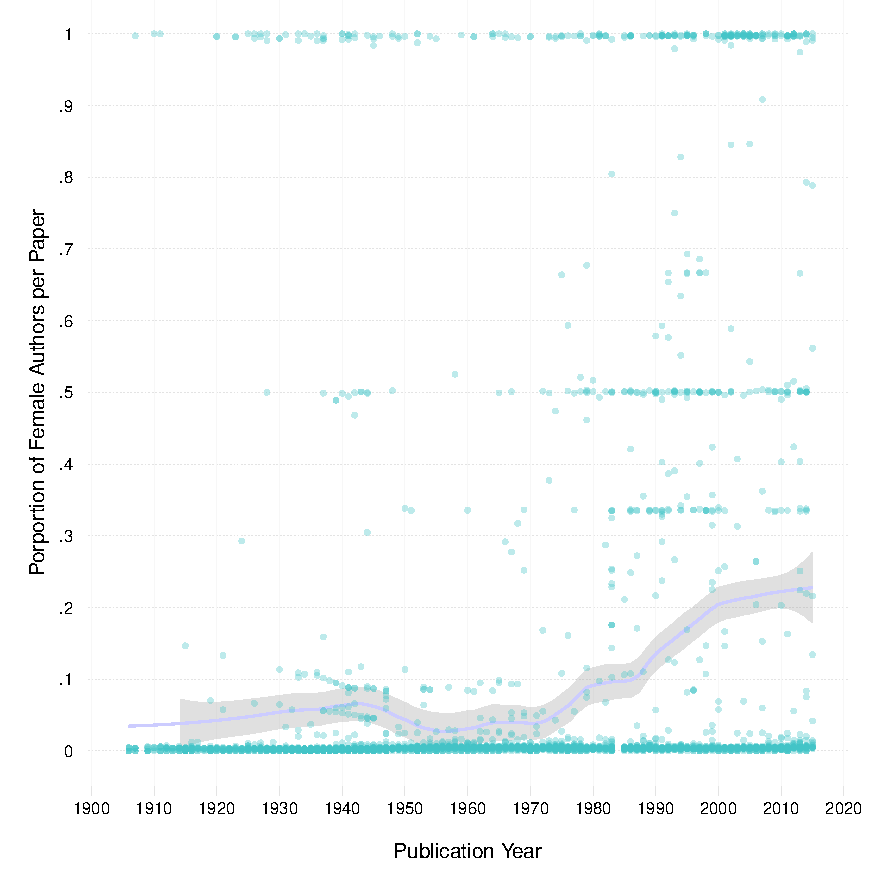
\includegraphics[scale=.85]{../figs/gender_authors_per_article_over_time.pdf}
\label{fig:women}
\end{figure}

\begin{figure}[htbp]
\centering
\caption{Abstract Views}
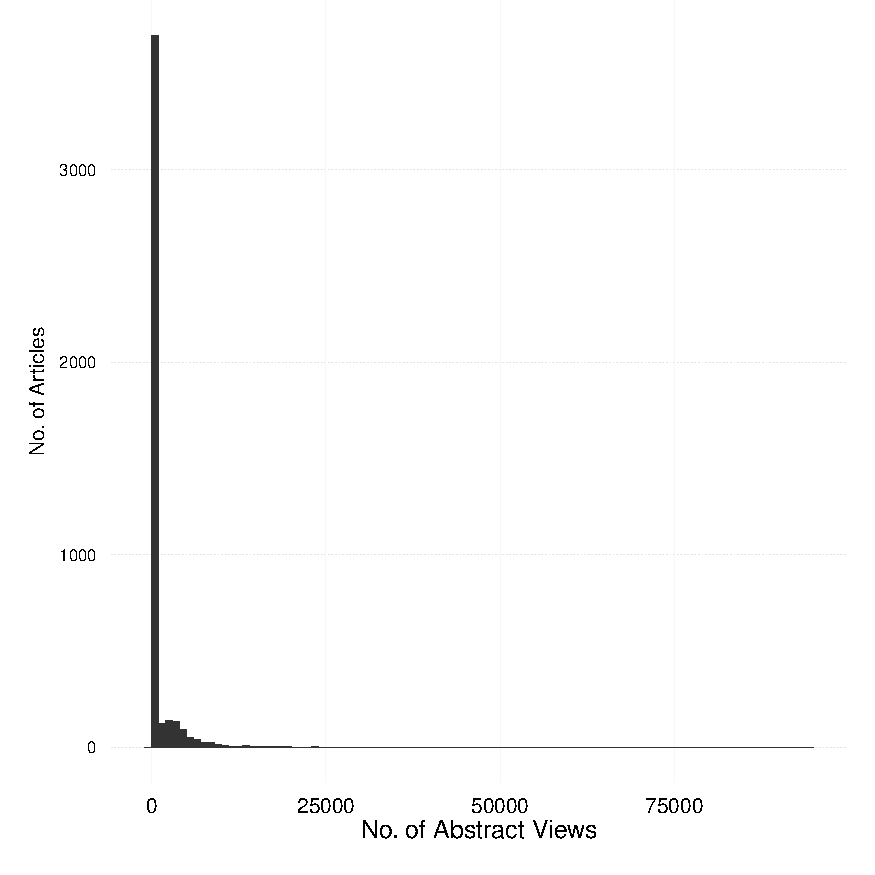
\includegraphics[scale=.85]{../figs/abstract_views.pdf}
\label{fig:abstracts}
\end{figure}

\begin{figure}[htbp]
\centering
\caption{Full-Text Views}
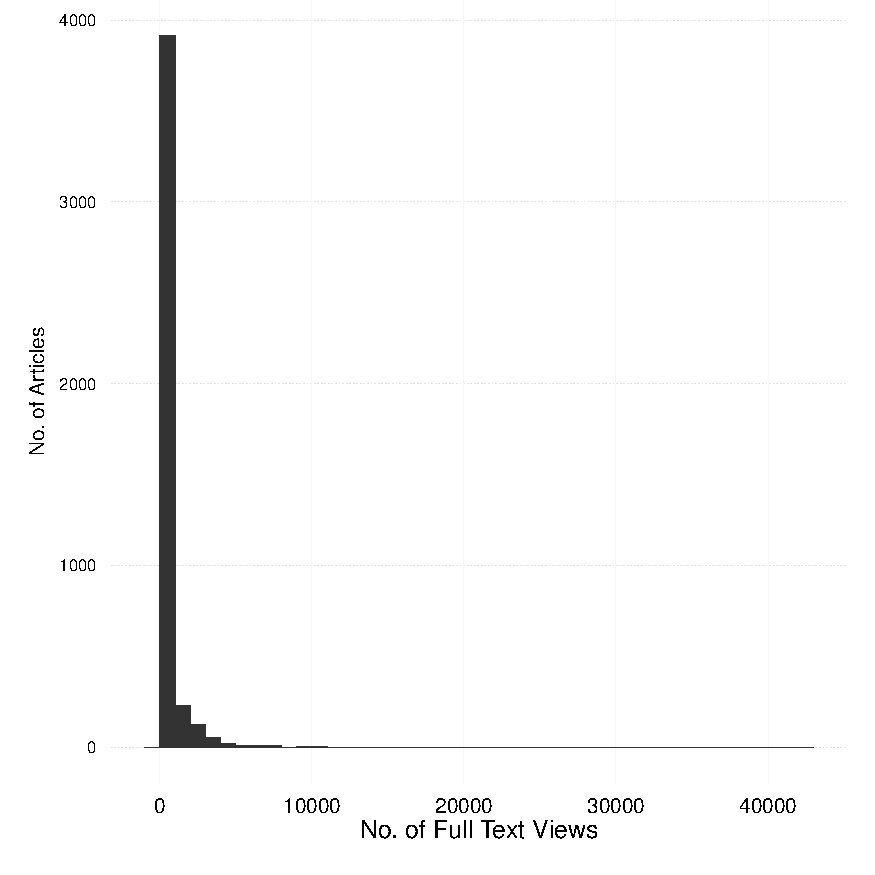
\includegraphics[scale=.85]{../figs/fulltext_views.pdf}
\label{fig:fulltext}
\end{figure}

\begin{figure}[htbp]
\centering
\caption{Title Length Over Time}
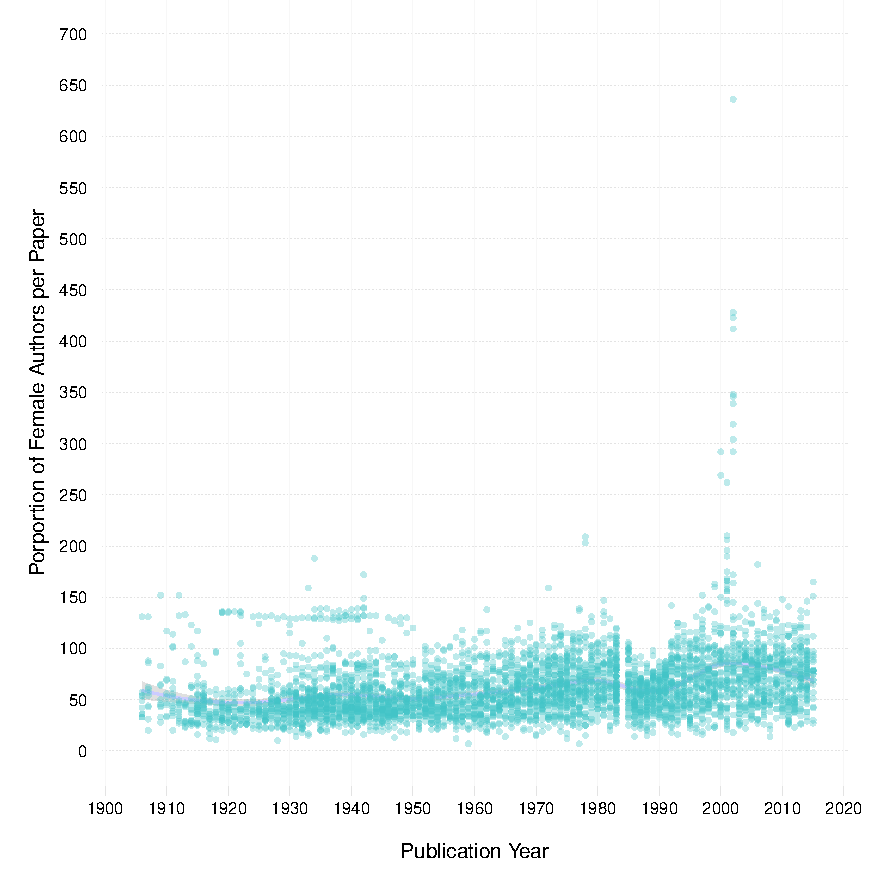
\includegraphics[scale=.85]{../figs/title_len_over_time.pdf}
\label{fig:fulltext}
\end{figure}

\clearpage
\bibliographystyle{apsr}
\bibliography{reviewbib}

\end{document}